\documentclass[11pt,a4paper]{article}

\usepackage[left=2cm,text={17cm,24cm},top=3cm]{geometry}
\usepackage[english]{babel}
\usepackage[utf8]{inputenc}
\usepackage[T1]{fontenc}
\usepackage{indentfirst}
\usepackage{hyperref}
\usepackage{float}

% URL
\usepackage{url}
\def\UrlBreaks{\do\/\do-}
\usepackage{breakurl}

% IMG
\usepackage{graphicx}
\graphicspath{{.}}

\usepackage{etoolbox}
\patchcmd{\thebibliography}{\section*{\refname}}{}{}{}

% #################################################################################################
\begin{document}
% #################################################################################################


% #################################################################################################
% TITLEPAGE
\begin{titlepage}
    \begin{center}
        \Huge
        \textsc{
            Faculty of Information Technology\\
            Brno University of Technology
        }
        \vspace{80px}
        \begin{figure}[!h]
            \centering
            
\includegraphics[scale=0.3]{img/vutbr-fit-logo.eps}
        \end{figure}
        \\[15mm]
        \Huge{
            \textbf{
                SEN
            }
        }
        \\[1.5mm]
        \huge{
            \textbf{
                Intelligent Sensors
            }
        }
        \\[2.5em]
        \LARGE{
            \textbf{
                Commissioning Heartbeat Sensor and Comparison\\
                Against Oximeter
            }
        }
        \vfill
    \end{center}
        \Large{
            \hfill\\
            Jiří Záleský (xzales12)\\
            Adrián Tóth (xtotha01)\hfill \today
        }

\end{titlepage}


% #################################################################################################
% CONTENT


\setlength{\parskip}{0pt}
\hypersetup{hidelinks}\tableofcontents
\setlength{\parskip}{0pt}

\newpage %#########################################################################################

\section{Abstract}

The goal of this project is to demonstrate a method of heart beat measurement via infrared light. The next sections below, will describe further details, which were required to be done to the right functionality. The results of measurement were compared with a valid heart beat sensor, which measured heart beat in other way than the infrared method.

\section{Introduction}

The necessary facilities for the implementation of the project were:\\[-1.5em]
\begin{itemize}
    \item Device shown in Figure \ref{fig:platform1}.
        \begin{figure}[H]
            \centering
            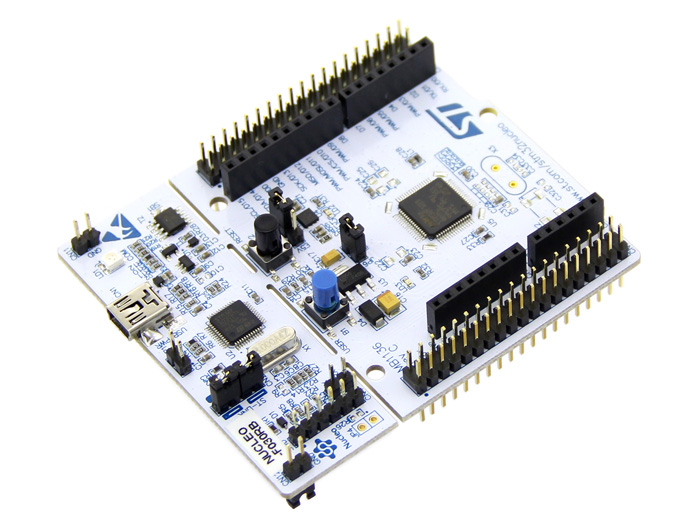
\includegraphics[scale=0.4]{img/device1.jpg}
            \caption{STM32 Nucleo board~\cite{IMG-DEVICE-1}.}
            \label{fig:platform1}
        \end{figure}
        \hfill\\[-17mm]
    \item Sensor shown in Figure \ref{fig:senzor1}.
        \begin{figure}[H]
            \centering
            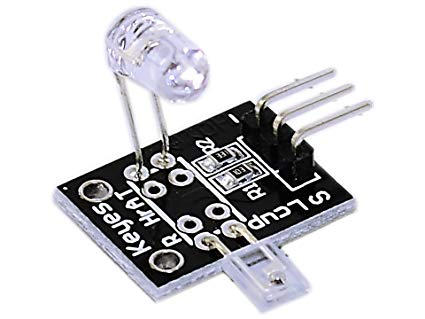
\includegraphics[scale=0.3]{img/sensor1.jpg}
            \caption{Keyes KY-039 Finger Heartbeat Detection Sensor~\cite{IMG-SENSOR-1}.}
            \label{fig:senzor1}
        \end{figure}
        \hfill\\[-18mm]
    \item Three female--to--female jumper wires.\\[-2.5mm]
\end{itemize}

\indent The device shown in Figure \ref{fig:platform1} - NUCLEO-F030R8~\cite{PLATFORM}, was the main platform for the project. The device was equipped with a STM32F030R8~\cite{MCU} microcontroller unit (MCU), which was designed and made to be suitable for a wide range of applications. MCU includes a set of peripherals through which it communicates with other devices such as the sensor shown in Figure \ref{fig:senzor1}. To create a communication pipeline, these units must be connected to each other via jumper wires. Wires provide a connection between the pins of units and so the pins have to be configured correctly.

\newpage %#########################################################################################

\section{Setup}

Firstly, the components must be connected to each other in a right way. Sensor, as a slave component shown in Figure \ref{fig:senzor2wires}, is connected to the main device (master component). These two units are connected via 3 jumper wires to the corresponding pins. The Figure \ref{fig:device2wires} and \ref{fig:senzor2wires} have three common marked pins: \textit{GND} (orange), \textit{5V} (yellow), \textit{PA0} (green); by which they are connected together. \textit{PA0} indicates an analog input pin to the master component. A precise description of all the necessary pins is shown in Figure \ref{fig:legend}.

\begin{figure}[H]
    \centering
    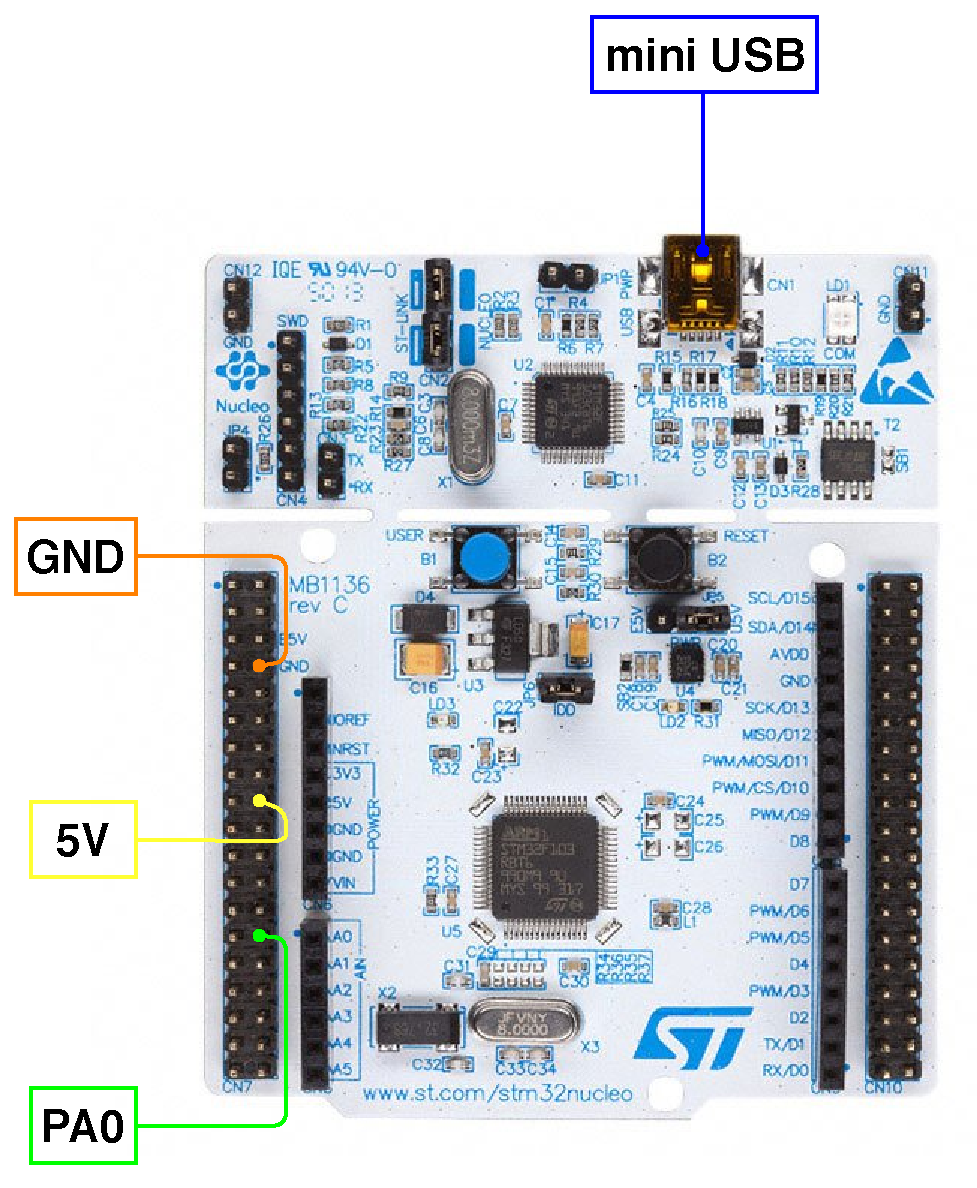
\includegraphics[scale=0.5]{img/device2-wires.pdf}
    \caption{NUCLEO-F030R8~\cite{IMG-DEVICE-2} connection scheme.}
    \label{fig:device2wires}
\end{figure}

\begin{figure}[H]
    \centering
    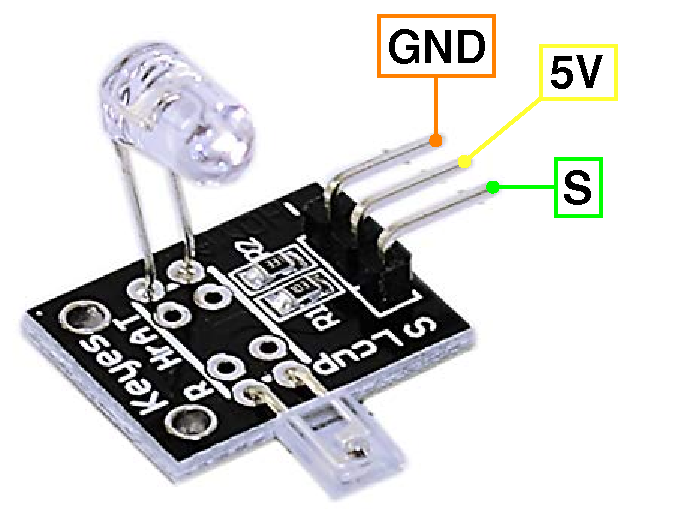
\includegraphics[scale=0.5]{img/sensor1-wires.pdf}
    \caption{Keyes KY-039~\cite{IMG-SENSOR-1} connection scheme relating to Figure \ref{fig:device2wires}.}
    \label{fig:senzor2wires}
\end{figure}

\begin{figure}[H]
    \begin{center}
        \begin{tabular}{|r|l|}
            \hline
            \textbf{B1} & button 1 \\
            \hline
            \textbf{B2} & button 2 \\
            \hline
            \textbf{LD2} & LED 2 \\
            \hline
            \textbf{GND} & ground \\
            \hline
            \textbf{5V} & 5 volt voltage supply \\
            \hline
            \textbf{PA0} & pin PA0 \\
            \hline
            \textbf{mini USB} & mini USB port \\
            \hline
        \end{tabular}
    \end{center}
    \caption{Explanatory notes.}
    \label{fig:legend}
\end{figure}

After proper connection of devices, which are attached to the computer via mini USB port (see Figure \ref{fig:connection}), they are ready to be programmed.

\begin{figure}[H]
    \centering
    
\includegraphics[scale=0.1]{img/vutbr-fit-logo.eps}
    \caption{Correct connection of devices.}
    \label{fig:connection}
\end{figure}

\section{Implementation}

...sensor code\cite{SENSOR}...

\section{Conclusion}

...

\newpage %#########################################################################################

\section{Appendix}

\begin{figure}[H]
    \begin{center}
        \begin{tabular}{|l|c|}
            \hline
            \textbf{Name} & \textbf{Value} \\
            \hline\hline
            n1 & v1 \\\hline
            n2 & v2 \\\hline
            n3 & v3 \\\hline
        \end{tabular}
    \end{center}
    \caption{Table of measurements.}
    \label{fig:measurements}
\end{figure}

\newpage %#########################################################################################

\section{References}
\bibliographystyle{englishiso}
\begin{flushleft}
    \bibliography{quotation}
\end{flushleft}


% #################################################################################################
\end{document}
% #################################################################################################
